\documentclass[border=5pt]{standalone}
\usepackage{pgfplots}
\usepackage{amsmath} % <-- This line is required

\pgfplotsset{compat=1.18}

\begin{document}

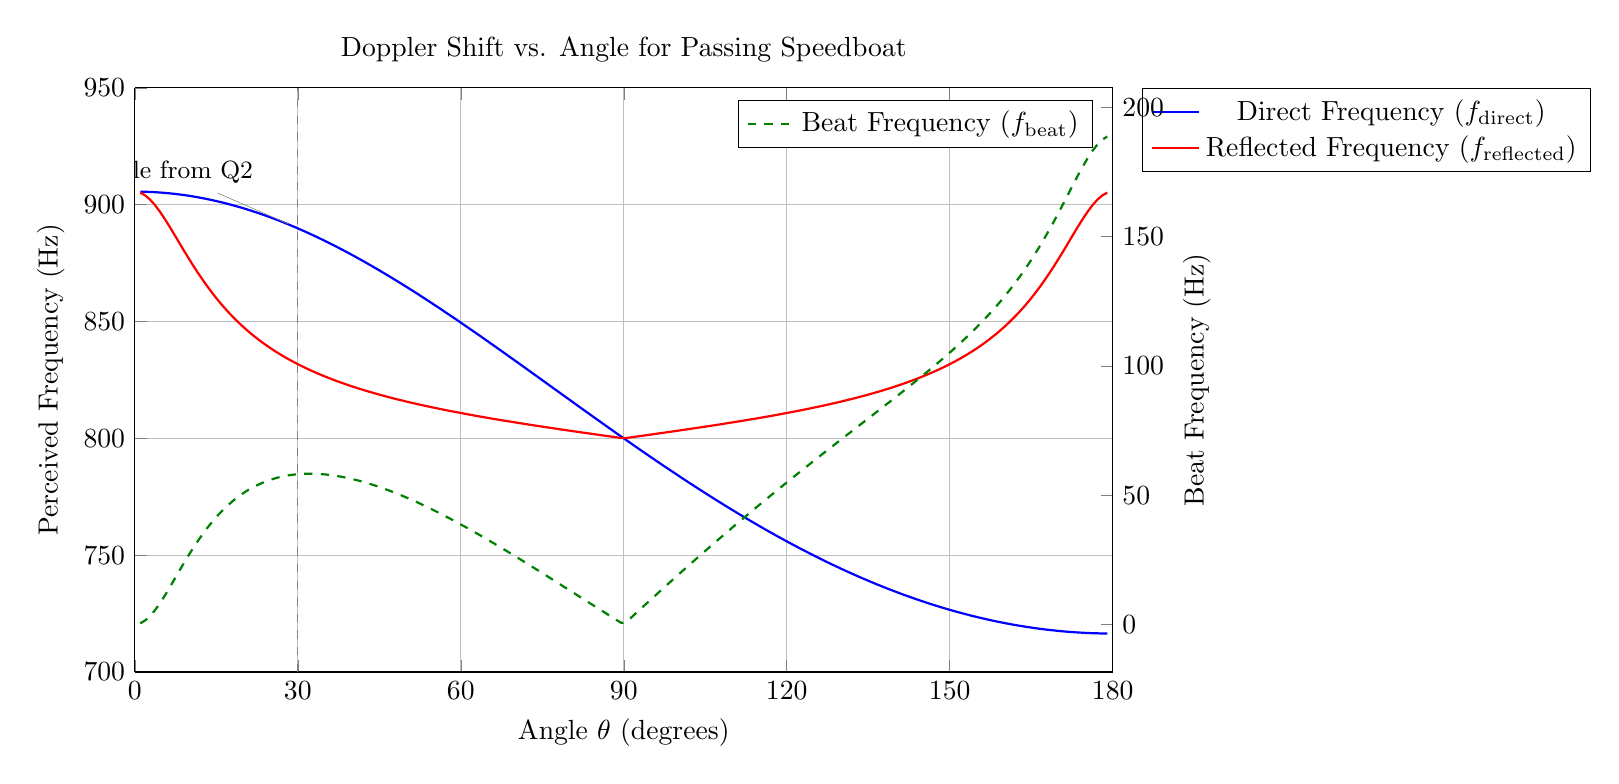
\begin{tikzpicture}
    \begin{axis}[
        width=14cm,
        height=9cm,
        title={Doppler Shift vs. Angle for Passing Speedboat},
        xlabel={Angle $\theta$ (degrees)},
        ylabel={Perceived Frequency (Hz)},
        xmin=0, xmax=180,
        ymin=700, ymax=950,
        xtick={0, 30, 60, 90, 120, 150, 180},
        grid=major,
        legend pos=outer north east,
        axis y line*=left, % Use left y-axis for the main plots
    ]

        % Plot the direct frequency using the explicit formula
        \addplot[
            domain=1:179, % Avoid 0 and 180 for tan() in the other plot
            samples=200,
            color=blue,
            thick,
        ] {800 * (343 / (343 - 40 * cos(x)))};
        \addlegendentry{Direct Frequency ($f_{\text{direct}}$)}

        % Plot the reflected frequency using its explicit formula
        \addplot[
            domain=1:179,
            samples=200,
            color=red,
            thick,
        ] {800 * (343 / (343 - 40 * cos(atan(5*tan(x)))))};
        \addlegendentry{Reflected Frequency ($f_{\text{reflected}}$)}

        % Add a vertical line to mark the angle from the original question
        \draw [dashed, gray] (axis cs:30, \pgfkeysvalueof{/pgfplots/ymin}) -- (axis cs:30, \pgfkeysvalueof{/pgfplots/ymax});
        \node[pin=135:{\small{Angle from Q2}}] at (axis cs:30, 890) {};

    \end{axis}

    \begin{axis}[
        width=14cm,
        height=9cm,
        xmin=0, xmax=180,
        axis y line*=right, % Use right y-axis for the beat frequency
        ylabel={Beat Frequency (Hz)},
        hide x axis, % Don't draw the x-axis twice
    ]
        % Plot the beat frequency using the explicit formulas
        \addplot[
            domain=1:179,
            samples=200,
            color=green!50!black,
            thick,
            dashed,
        ] {abs( (800 * (343 / (343 - 40 * cos(x)))) - (800 * (343 / (343 - 40 * cos(atan(5*tan(x))))) ) )};
        \addlegendentry{Beat Frequency ($f_{\text{beat}}$)}
    \end{axis}

\end{tikzpicture}

\end{document}